\documentclass{article}

\usepackage{physics} % Handy shortcuts like \pdv, \dd and much more
\usepackage[top=1.5cm]{geometry} % smaller margins, can be adjusted if given arguments
\usepackage{siunitx} % the \si environment for units
\usepackage{mathtools} % The dcases environment, prettier than just cases
\usepackage{tikz} % For drawing picures
\usepackage{wrapfig} % Wrapping text around figures
\usepackage{enumitem} % Getting alphabetical enumerate


\title{Exercise 9 - TFY4345 Classical Mechanics}
\date{2020}

\begin{document}
    \maketitle
    \begin{wrapfigure}{2}{0.3\textwidth}
        \vspace{-0.5cm}
        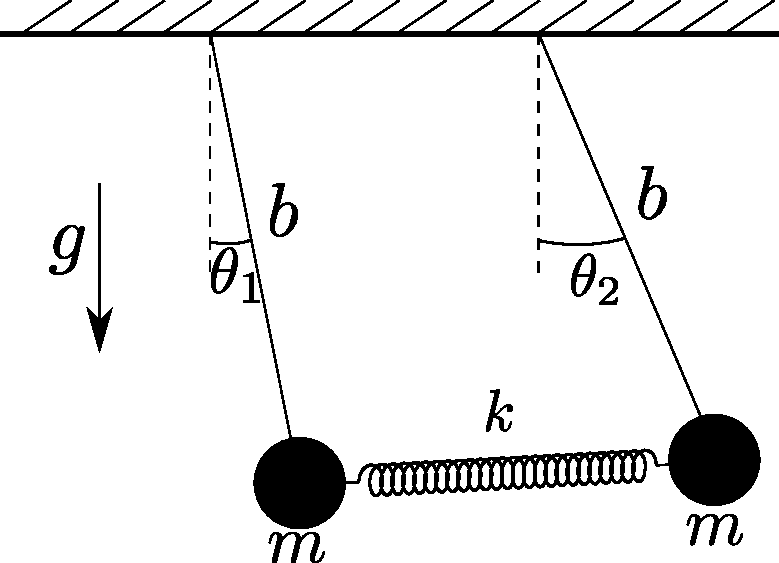
\includegraphics[width=0.3\textwidth]{figures/figure_1.pdf}
        \vspace*{-2.1cm}
    \end{wrapfigure}
    \section{Coupled pendula}
    Consider the system of two pendula of length $b$, with masses $m$ and coupled by a spring with spring constant $k$. The spring is unstretched in the equilibrium position $\theta_1 = \theta_2 = 0$. Start by writing down the kinetic and potential energy of the system in generalized coordinates. Determine the eigenfrequencies and describe the normal mode motion of the system. Assume small oscillations.

    \section{Two coupled oscillators}
    \begin{wrapfigure}{2}{0.35\textwidth}
        \vspace{-0.5cm}
        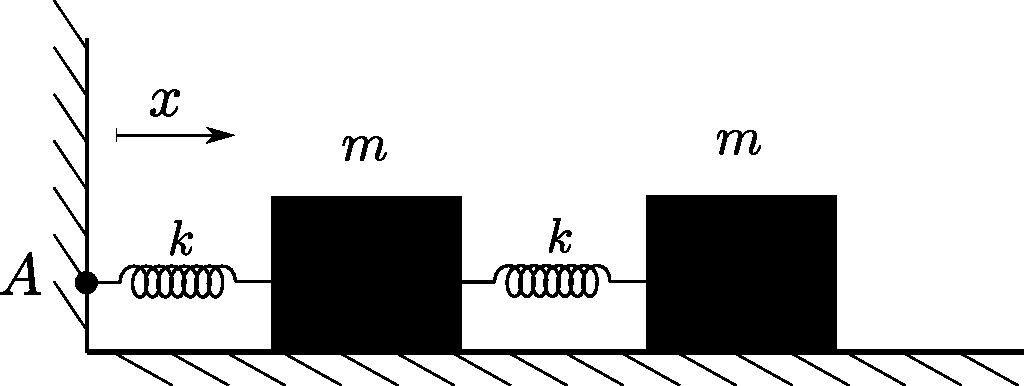
\includegraphics[width=0.35\textwidth]{figures/figure_2.pdf}
        \vspace*{-1.5cm}
    \end{wrapfigure}
    Evaluate the eigenfrequencies of the system of two masses $m$, attached to each other by and a fixed point $A$ by two springs with spring constant $k$ as shown in the figure. Determine the associated eigenfrequencies, and describe the vibrational modes qualitatively. Assume the masses glide without friction.

    \section{Oscillating body with two attached pendula}
    \begin{wrapfigure}{2}{0.3\textwidth}
        \vspace{-0.5cm}
        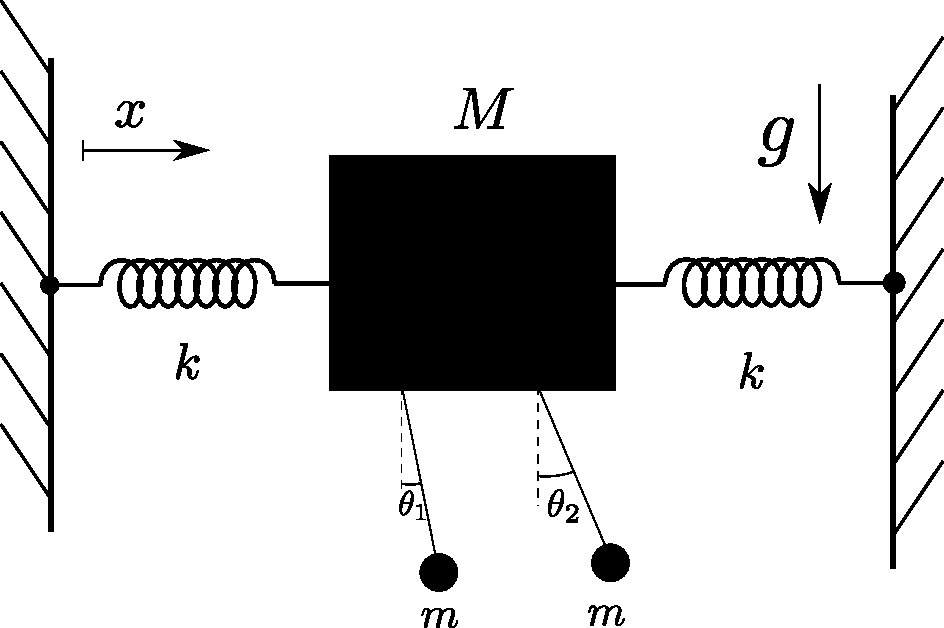
\includegraphics[width=0.3\textwidth]{figures/figure_3.pdf}
        \vspace{-1.5cm}
    \end{wrapfigure}
    Consider a block of mass $M$, attached by two springs of equal spring constants $k$ on opposite sides to a wall. The mass has two pendula of mass $m$ and length $\ell$ attached to the underside. Assume small oscillations, and evaluate the eigenfrequencies of the system. You will need three generalized coordinates.

    \section{Double pendulum}
    \begin{wrapfigure}{2}{0.15\textwidth}
        \vspace{-0.5cm}
        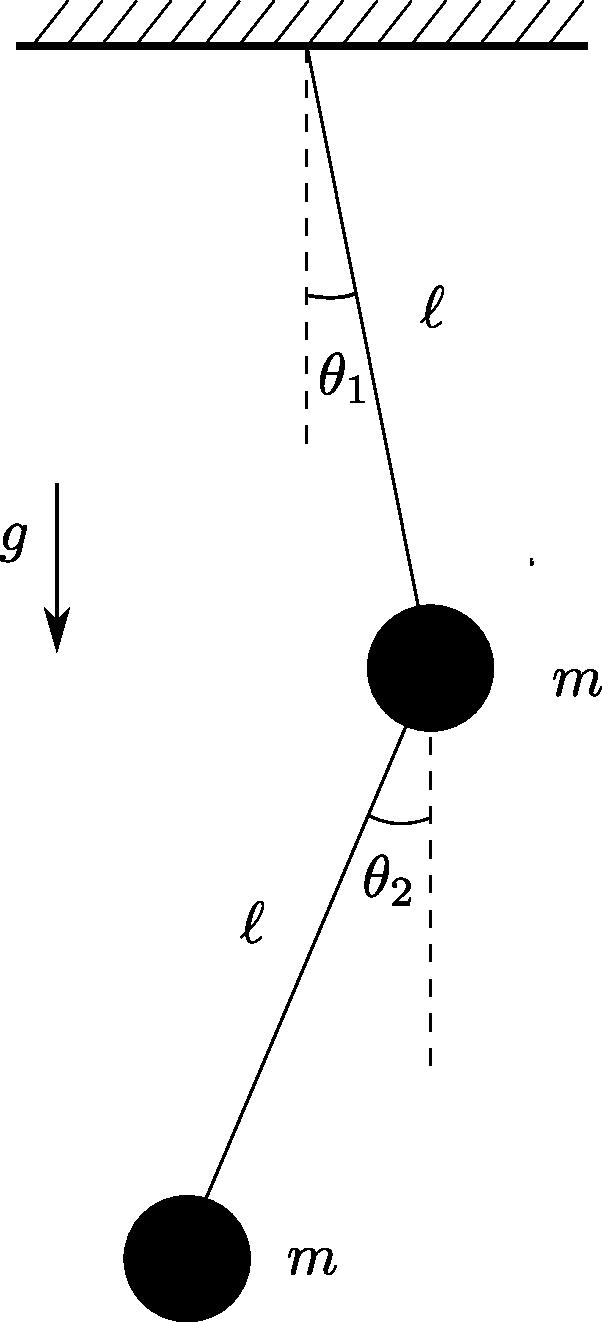
\includegraphics[width=0.15\textwidth]{figures/figure_4.pdf}
    \end{wrapfigure}
    Consider a double pendulum with equal masses $m$ and of equal lengths $\ell$. Assume small oscillation, and determine the eigenfrequencies and eigenvectors based on the theory of couple oscillations.

\end{document}
